\section{Object Storage}
In Calico, all core components are stored using high performance Java hash maps. 
We decided that using FastUtil's\cite{fastutil} high performance maps would provide a better response time as opposed to using Java's core HashMap class. 
Each controller contains a single hash map that acts as a database for all objects that the controller is responsible for.
All access to hash maps requires use of a ``key'' to perform a lookup.
All objects are given a sequential 64-bit integer that acts as a globally unique identifier for each object.

One important design decision that was made was the choice to use a sequential identifier for each new object. The two factors that influenced our decision were: the relatively small size of a 64-bit integer in comparison with a universally unique string (which would be almost double the size), and better client performance.
Small size was very important to us - this identifier would be included in nearly every network packet that was sent to and from the server. We wanted the footprint to be as small as possible, but we needed something that we could ensure would be unique for every object. 
The second decision - better client performance - was another benefit provided by using a sequential identifier. Clients could request a pre-allocated block of identifiers that they could assign to objects created client-side. The client could then create objects and assign them an identifier and submit the object directly to the server. Due to the fact that identifiers were pre-allocated, the client did not have to wait for confirmation from the server in order to add the object to its local hash map.

\begin{figure}[htb]
  \centering
  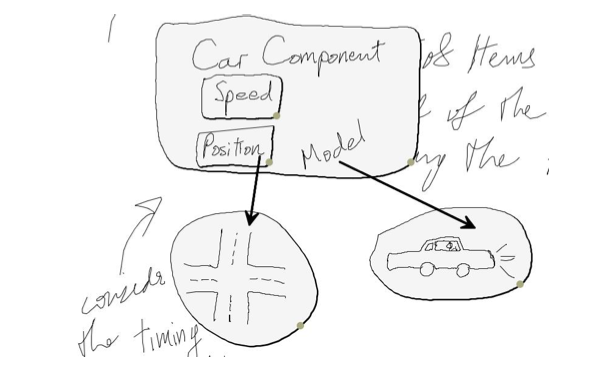
\includegraphics[width=0.8\textwidth]{scraps.png}
  \label{fig:scraps_storage}
\end{figure}

The screenshot shown above displays a typical design session in Calico. The content shown above would be stored in the various databases within each controller. This image represents a single \texttt{Canvas} object which would be stored within the \texttt{CanvasController} class. The \texttt{Canvas} object would have a list that contains the identifiers for each object that is being displayed on screen (five \texttt{Scrap}s, two \texttt{Arrow}s, and many \texttt{Stroke}s). Each of these objects would be stored in their respective controller. Each of these objects would require a list of \texttt{Point}s that would form the boundaries of the object. These are used within Calico to determine the location of an object, as well as whether an object is ``contained'' within another object (such as a scrap). Each object can have additional attributes that are specific to its type (arrows would need endpoints, strokes would have a color). These attributes would be stored within the object itself and would be converted to a \texttt{CalicoPacket} whenever a new client connected and needed to load the existing state of Calico.

